\documentclass[sigconf]{acmart}

%%
%% \BibTeX command to typeset BibTeX logo in the docs
\AtBeginDocument{%
  \providecommand\BibTeX{{%
    \normalfont B\kern-0.5em{\scshape i\kern-0.25em b}\kern-0.8em\TeX}}}

%% Rights management information.  This information is sent to you
%% when you complete the rights form.  These commands have SAMPLE
%% values in them; it is your responsibility as an author to replace
%% the commands and values with those provided to you when you
%% complete the rights form.
\setcopyright{acmcopyright}
\copyrightyear{2018}
\acmYear{2018}
\acmDOI{10.1145/1122445.1122456}

%% These commands are for a PROCEEDINGS abstract or paper.
\acmConference[FPGA'19]{International Symposium on Field-Programmable Gate Arrays}{February 23--25, 2019}{Monterey, CA, USA} 
\acmYear{2019}
\acmBooktitle{FPGA '19: International Symposium on Field-Programmable Gate Arrays,
  February 23--25, 2019, Monterey, CA}
\acmPrice{15.00}
\acmISBN{978-1-4503-9999-9/18/06}


%%
%% Submission ID.
%% Use this when submitting an article to a sponsored event. You'll
%% receive a unique submission ID from the organizers
%% of the event, and this ID should be used as the parameter to this command.
%%\acmSubmissionID{123-A56-BU3}

%%
%% The majority of ACM publications use numbered citations and
%% references.  The command \citestyle{authoryear} switches to the
%% "author year" style.
%%
%% If you are preparing content for an event
%% sponsored by ACM SIGGRAPH, you must use the "author year" style of
%% citations and references.
%% Uncommenting
%% the next command will enable that style.
%%\citestyle{acmauthoryear}

%%
%% end of the preamble, start of the body of the document source.

%%%%%%%%%%%%%%%%%%%%%%%%%%%%%%%%%%%%%%%%%%%%%%%%%%%%%%%%%%%%%%%%%%%%%%%%%%%%%%%%%%
% Packages & Macros
%%%%%%%%%%%%%%%%%%%%%%%%%%%%%%%%%%%%%%%%%%%%%%%%%%%%%%%%%%%%%%%%%%%%%%%%%%%%%%%%%%
\usepackage{booktabs} % For formal tables
\graphicspath{{./graphics/}}
\DeclareGraphicsExtensions{.pdf,.jpeg,.png}


% *** GRAPHICS RELATED PACKAGES ***
%
%\usepackage[pdftex]{graphicx}

\usepackage[export]{adjustbox}
\usepackage{color}


% *** MATH PACKAGES ***
%
\usepackage{amsmath}
\usepackage{amssymb}
% A popular package from the American Mathematical Society that provides
% many useful and powerful commands for dealing with mathematics.
%
% Note that the amsmath package sets \interdisplaylinepenalty to 10000
% thus preventing page breaks from occurring within multiline equations. Use:
%\interdisplaylinepenalty=2500
% after loading amsmath to restore such page breaks as IEEEtran.cls normally
% does. amsmath.sty is already installed on most LaTeX systems. The latest
% version and documentation can be obtained at:
% http://www.ctan.org/pkg/amsmath




% *** ALIGNMENT PACKAGES ***
%
\usepackage{array}
% Frank Mittelbach's and David Carlisle's array.sty patches and improves
% the standard LaTeX2e array and tabular environments to provide better
% appearance and additional user controls. As the default LaTeX2e table
% generation code is lacking to the point of almost being broken with
% respect to the quality of the end results, all users are strongly
% advised to use an enhanced (at the very least that provided by array.sty)
% set of table tools. array.sty is already installed on most systems. The
% latest version and documentation can be obtained at:
% http://www.ctan.org/pkg/array


% *** FLOAT PACKAGES ***
%
\usepackage{fixltx2e}
% fixltx2e, the successor to the earlier fix2col.sty, was written by
% Frank Mittelbach and David Carlisle. This package corrects a few problems
% in the LaTeX2e kernel, the most notable of which is that in current
% LaTeX2e releases, the ordering of single and double column floats is not
% guaranteed to be preserved. Thus, an unpatched LaTeX2e can allow a
% single column figure to be placed prior to an earlier double column
% figure.
% Be aware that LaTeX2e kernels dated 2015 and later have fixltx2e.sty's
% corrections already built into the system in which case a warning will
% be issued if an attempt is made to load fixltx2e.sty as it is no longer
% needed.
% The latest version and documentation can be found at:
% http://www.ctan.org/pkg/fixltx2e



% *** NON FLOAT MINIPAGE ***
\makeatletter
\let\MYcaption\@makecaption
\makeatother

\usepackage{caption}
\usepackage[font=footnotesize]{subcaption}

\usepackage[inline]{enumitem}

\makeatletter
\let\@makecaption\MYcaption
\makeatother


% *** PDF, URL AND HYPERLINK PACKAGES ***
%
%\usepackage{hyperref}
\usepackage{url}
% url.sty was written by Donald Arseneau. It provides better support for
% handling and breaking URLs. url.sty is already installed on most LaTeX
% systems. The latest version and documentation can be obtained at:
% http://www.ctan.org/pkg/url
% Basically, \url{my_url_here}.


% *** MINTED COLORED CODE ***
\usepackage{minted} % Required to display colored code properly
%hack for minted to get rid of syntax error boxes
\makeatletter
\AtBeginEnvironment{minted}{\dontdofcolorbox}
\def\dontdofcolorbox{\renewcommand\fcolorbox[4][]{##4}}
\makeatother
\usepackage[utf8]{inputenc}

% *** Do not adjust lengths that control margins, column widths, etc. ***
% *** Do not use packages that alter fonts (such as pslatex).         ***
% There should be no need to do such things with IEEEtran.cls V1.6 and later.
% (Unless specifically asked to do so by the journal or conference you plan
% to submit to, of course. )

\usepackage{algorithm}
\usepackage{algorithmic}

% *** Custom Frame ***
\usepackage{mdframed}

% So footnotes for figures are properly placed
\usepackage{afterpage}

% correct bad hyphenation here
\hyphenation{op-tical net-works semi-conduc-tor}

% for left justification of text
\usepackage{ragged2e}

% for footnotes inside tables
\usepackage{threeparttable}
% helpful macros

\usepackage{xspace}

\newcommand{\hide}[1]{}
\setlength{\marginparwidth}{2cm}
%\newcommand{\comment}[1]{\marginpar{\footnotesize #1}}
%\newcommand{\comment}[1]{}
\newcommand{\comment}[1]{\textcolor{red}{[#1]}}
\renewcommand{\tilde}[0]{$\sim$}
\newcommand{\us}[0]{$\mu s$}

\newcommand{\fig}[1]{Fig.~\ref{#1}\xspace}
\newcommand{\tbl}[1]{Table~\ref{#1}\xspace}
\newcommand{\sect}[1]{Section~\ref{#1}\xspace}

% affiliation shorthand
\newcommand{\ee}[0]{$^{1}$}
\newcommand{\cs}[0]{$^{2}$}
\newcommand{\eecs}[0]{$^{1,2}$}
\definecolor{code-bgnd}{gray}{0.95}
\newcommand{\code}[1]{\colorbox{code-bgnd}{\texttt{#1}}}
%%%%%%%%%%%%%%%%%%%%%%%%%%%%%%%%%%%%%%%%%%%%%%%%%%%%%%%%%%%%%%%%%%%%%%%%%%%%%%%%%%

\begin{document}

%%%%%%%%%%%%%%%%%%%%%%%%%%%%%%%%%%%%%%%%%%%%%%%%%%%%%%%%%%%%%%%%%%%%%%%%%%%%%%%%%%
% Graphics Sources
%%%%%%%%%%%%%%%%%%%%%%%%%%%%%%%%%%%%%%%%%%%%%%%%%%%%%%%%%%%%%%%%%%%%%%%%%%%%%%%%%%
\graphicspath{{./graphics/}}
\DeclareGraphicsExtensions{.pdf,.jpeg,.png}
%%%%%%%%%%%%%%%%%%%%%%%%%%%%%%%%%%%%%%%%%%%%%%%%%%%%%%%%%%%%%%%%%%%%%%%%%%%%%%%%%%


%%%%%%%%%%%%%%%%%%%%%%%%%%%%%%%%%%%%%%%%%%%%%%%%%%%%%%%%%%%%%%%%%%%%%%%%%%%%%%%%%%
% Title & Authors
%%%%%%%%%%%%%%%%%%%%%%%%%%%%%%%%%%%%%%%%%%%%%%%%%%%%%%%%%%%%%%%%%%%%%%%%%%%%%%%%%%
%% The "title" command has an optional parameter,
%% allowing the author to define a "short title" to be used in page headers.
\title{Hardware Description Beyond Register-Transfer Level Languages}

%%
%% The "author" command and its associated commands are used to define
%% the authors and their affiliations.
%% Of note is the shared affiliation of the first two authors, and the
%% "authornote" and "authornotemark" commands
%% used to denote shared contribution to the research.

\author{Oron Port}
\email{soronpo@campus.technion.ac.il}
\affiliation{%
  \institution{Technion -- Israel Institute of Technology}
  \city{Haifa}
  \state{Israel}
}

\author{Yoav Etsion}
\email{yetsion@technion.ac.il}
\affiliation{%
	\institution{Technion -- Israel Institute of Technology}
	\city{Haifa}
	\state{Israel}
}
%%
%% By default, the full list of authors will be used in the page
%% headers. Often, this list is too long, and will overlap
%% other information printed in the page headers. This command allows
%% the author to define a more concise list
%% of authors' names for this purpose.
%\renewcommand{\shortauthors}{Trovato and Tobin, et al.}
%%%%%%%%%%%%%%%%%%%%%%%%%%%%%%%%%%%%%%%%%%%%%%%%%%%%%%%%%%%%%%%%%%%%%%%%%%%%%%%%%%



%%%%%%%%%%%%%%%%%%%%%%%%%%%%%%%%%%%%%%%%%%%%%%%%%%%%%%%%%%%%%%%%%%%%%%%%%%%%%%%%%%
% Abstract & Keywords
%%%%%%%%%%%%%%%%%%%%%%%%%%%%%%%%%%%%%%%%%%%%%%%%%%%%%%%%%%%%%%%%%%%%%%%%%%%%%%%%%%
%% The abstract is a short summary of the work to be presented in the
%% article.
% As a general rule, do not put math, special symbols or citations
% in the abstract
\begin{abstract}
Today's dominant hardware description languages (HDLs), namely Verilog and VHDL, rely on limited register-transfer-level (RTL) constructs. These constructs tightly couple design functionality with timing requirements and target-device constraints. As hardware designs and device architectures become increasingly more complex, these dominant HDLs yield verbose and unportable code.
To raise the level of abstraction, several high-level synthesis (HLS) tools were introduced, usually based on software languages such as C. Unfortunately, designing hardware with sequential software language semantics comes at a price; the designer loses the ability to control hardware construction and data scheduling, which is crucial in many design use-cases. 

In this paper we further extend DFiant, a Scala-based HDL that uses the dataflow model to decouple functionality from implementation constraints.
DFiant's frontend enables functional bit-accurate hardware description, while maintaining a complete timing-agnostic and device-agnostic code. DFiant bridges the gap between software programming and hardware construction, driving an intuitive functional object oriented code into a high-performance hardware implementation.

For a proof of concept, we implemented a compiler frontend for DFiant, which transforms DFiant code into a dataflow graph, and a preliminary auto-pipelining backend, which maps the graph into synthesizable Verilog code. We further implemented two test cases in DFiant: an Advanced Encryption Standard cipher block and an IEEE-754 floating point multiplier. We compared both test cases against modern design flows. Our results demonstrate that DFiant can greatly simplify hardware designs yet still maintain competitive performance.
\end{abstract}

%We defined a new language from the ground up, borrowing concepts from hardware, dataflow and software languages. The result is a strongly-typed, purely synthesizable extendable language frontend, fit for both general-purpose and high level hardware description.

%%
%% The code below is generated by the tool at http://dl.acm.org/ccs.cfm.
%% Please copy and paste the code instead of the example below.
%%
 \begin{CCSXML}
	<ccs2012>
	<concept>
	<concept_id>10010583.10010682.10010689</concept_id>
	<concept_desc>Hardware~Hardware description languages and compilation</concept_desc>
	<concept_significance>500</concept_significance>
	</concept>
	</ccs2012>
\end{CCSXML}

\ccsdesc[500]{Hardware~Hardware description languages and compilation}

%%
%% Keywords. The author(s) should pick words that accurately describe
%% the work being presented. Separate the keywords with commas.
\keywords{HDL, HLS, Dataflow}
%%%%%%%%%%%%%%%%%%%%%%%%%%%%%%%%%%%%%%%%%%%%%%%%%%%%%%%%%%%%%%%%%%%%%%%%%%%%%%%%%%


%% A "teaser" image appears between the author and affiliation
%% information and the body of the document, and typically spans the
%% page.
%\begin{teaserfigure}
%  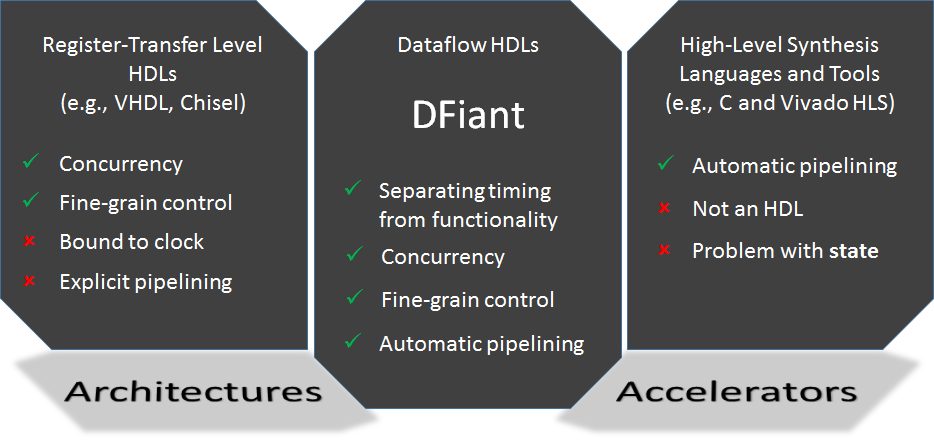
\includegraphics[width=\textwidth]{graphics/teaser}
%  \caption{DFiant bridges the gap}
%  \label{fig:teaser}
%\end{teaserfigure}

%%
%% This command processes the author and affiliation and title
%% information and builds the first part of the formatted document.
\maketitle

%%%%%%%%%%%%%%%%%%%%%%%%%%%%%%%%%%%%%%%%%%%%%%%%%%%%%%%%%%%%%%%%%%%%%%%%%%%%%%%%%%
% Sections
%%%%%%%%%%%%%%%%%%%%%%%%%%%%%%%%%%%%%%%%%%%%%%%%%%%%%%%%%%%%%%%%%%%%%%%%%%%%%%%%%%
\section{Introduction}
The register-transfer level (RTL) programming model paved the road for Verilog and VHDL to flourish as the leading hardware description languages (HDLs). That road, however, is steadily nearing its end as both hardware designs and devices become increasingly more complex. While the software world is striving for a "write once, run anywhere" programmability, the complexity of an RTL design implementing a given functionality may vary greatly across different FPGA and ASIC devices that incorporate various technologies and core components. Moreover, minor requirement changes may lead to significant redesigns, since RTL abstraction tightly couples functionality with timing constraints. For example, registers serve various roles such as preserving a state, pipelining and balancing a data path, deriving timed signals from an input clock, and synchronizing an input signal. This coupling between functionality, timing constraints, and device constraints leads to verbose and unportable RTL designs. 

\begin{figure}[h]
	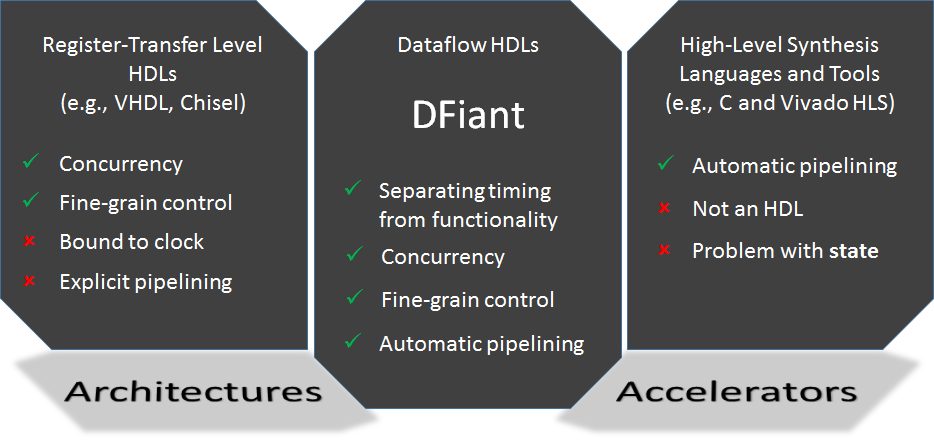
\includegraphics[width=\linewidth]{graphics/teaser}
	\caption{DFiant bridges the gap}
	\label{fig:teaser}
\end{figure}

Ongoing efforts to bridge this hardware programmability gap~\cite{Kapre2016, Nane2016, Windh2015} can be largely split into two classes: high-level synthesis (HLS) tools and high-level RTL (HL-RTL) languages.
On the one hand, HLS tools (such as Vivado~\cite{Vivado2012}, Catapult~\cite{graphics2008catapult}, and others~\cite{Kavvadias2013, synphony2015}) rely on programming languages like C and incorporate auto-pipelining and optimization mechanisms to make hardware accelerators accessible for non-hardware engineers. While this approach is successful in algorithmic acceleration domains, such languages carry von Neumann sequential semantics and thus hinder construction of parallel hardware, which is crucial for hardware design~\cite{Zhao2017}. Moreover, some trivial periodic hardware operations (like toggling a LED) are unbearably difficult to implement in HLS languages.
On the other hand, HL-RTL languages (such as Chisel~\cite{Bachrach2012}, Bluespec~\cite{nikhil2004bluespec}, PyRTL~\cite{Clow2017}, and others~\cite{Charles2016, Liu2017, jiang2018mamba, decaluwe2004myhdl, CxLang2014, Lockhart2014}) aim to enhance productivity by introducing new hardware generation constructs and semantics but do not abstract away register-level description (even Bluespec, which uses concurrent guarded atomic actions, assumes rules complete within a single clock cycle). Therefore, HL-RTL designs are still subjected to the \emph{"tyranny of the clock"}~\cite{Sutherland2012} and are bound to specific timing and target constraints.

In this paper we propose dataflow-based HDL constructs that abstract away registers and clocks. We further introduce DFiant\footnote{A preliminary version of DFiant was first introduced as a poster. The reference was removed for blind review.}, a Scala-embedded HDL that utilizes these dataflow constructs to decouple functionality from implementation constraints. DFiant brings together constructs and semantics from dataflow~\cite{le1986signal, Thuau1991, gurd1985manchester, arvind1992id}, hardware, and software programming languages to enable truly portable and composable hardware designs. The dataflow model offers implicit concurrency between independent paths while freeing the designer from explicit register placement that binds the design to fixed pipelined paths and timing constraints.

\begin{figure*}[t]
	\centering
	\captionsetup{justification=centering}
	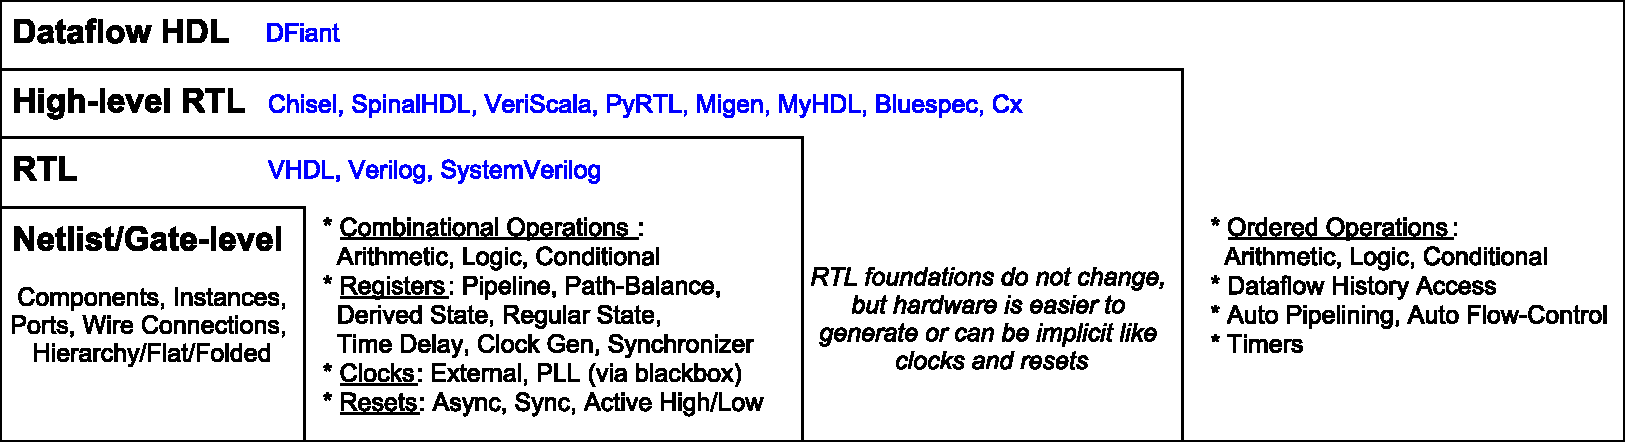
\includegraphics[width=\linewidth]{graphics/motivation.pdf} 
	\captionof{figure}{HDL abstraction layer summary (lowest=netlist, highest=dataflow)\\ Each layer subsumes the capabilities of the layer below it. Dataflow constructs replace RTL registers with their true functionality (e.g., state) or inserts them implicitly (e.g., pipelining). }
	\label{fig:motivation}
\end{figure*}

Recent related dataflow-for-hardware efforts are the Maxeler framework~\cite{Pell2011} and its MaxJ Java-based programming language, the OpenDF framework~\cite{bhattacharyya2008opendf} which is based on the CAL actor language~\cite{eker2003cal}, and CAPH~\cite{serot2011implementing}. MaxJ indeed shares common traits with DFiant, but it is tailored for its target hardware framework and is not designed to be a general purpose HDL. Both OpenDF and CAPH share similar goals with our work, but they use actors and networks to describe hardware, which is completely different than a conventional HDL composition based on component instances and port connections.

This work focuses on applying dataflow principles through the DFiant language and compiler. DFiant is \emph{not} an HLS language, nor is it an RTL language. Instead, DFiant is an HDL that provides abstractions beyond the RTL behavioral model, which reduce verbosity and maintain portable code. Since DFiant is implemented as a Scala library, it offers a rich type safe ecosystem alongside its own hardware-focused type system (e.g., bit-accurate dataflow types, input/output port types). The library performs two main tasks: first, the frontend compilation, which enforces the type-safe rule-system and constructs a dataflow dependency graph; and second, the backend compilation, which translates the graph into a pipelined RTL code and a TCL constraints file. The resulting code can be synthesized using commercial tools. 

The remainder of this paper is organized as follows. The next section details the motivation behind the dataflow HDL abstractions, and Section~\ref{sec:dfiant} which provides a general overview of the DFiant HDL language. 
Section~\ref{sec:evaluation} describes our evaluation of the DFiant language and compiler, and, finally, Section~\ref{sec:conclusion} concludes the paper.


%Interactions between DFiant types lead to hardware construction, while non-DFiant types (e.g. Integer) are considered as constants. 
 
\section{A Dataflow Hardware Description Abstraction}
\label{sec:motivation}
In this section we detail how dataflow abstraction, when applied to an HDL, helps to decouple the function from its constraints. We also describe generally what dataflow HDL constructs are required to achieve maximum portable code, and in the next section we specifically demonstrate these constructs take effect in DFiant.

\fig{fig:motivation} summarizes the basic elements that make up HDLs at different abstraction layers, from the lowest layer, a netlist, to the dataflow HDL layer presented in this paper. Each layer includes the expressive capabilities of the lowest layer (e.g., structural instance composition is possible in all HDLs). The layers are tagged with the relevant HDL names. Note that HLS languages and simulation constructs are not included in this summary. 

The basic notion of a dataflow abstraction is that instead of wires and registers we have dataflow token streams. This key difference between RTL and dataflow abstractions reveal why one is coupled to the device and timing constraints while the other is agnostic to them. Firstly, the RTL abstraction utilizes combinational operations that must complete (their propagation delay) within a given cycle if fed to a register, while the dataflow abstraction only assumes order and not exactly when the operations are to complete. This decoupling from fixed clock cycles leaves the option to pipeline the operations at will. Secondly, the RTL abstraction directly uses registers for variety of other reasons, thus binds the design to specific timing conditions, while the dataflow abstraction provides higher constructs to avoid specific clock binding where possible. We classify the various register use-cases, and present their dataflow abstracted counterpart. The classifications are divided into three main categories: \textit{synchronous technology backend}, \textit{synchronous technology interface}, and \textit{state}.

\subsection{Synchronous Technology Backend}
Registers are often forced upon the design due to a synchronous technology choice. Since they are unrelated to the functional requirement, a dataflow HDL requires no constructs to express them and relies on its compiler to implement them properly based on the functional requirements and design constraints. 
We differentiate between the following backend register uses:
\subsubsection{Pipelining and Path-Balancing}
Pipeline registers are inserted to split long combinational paths and their placement is determined by designer-specified constraints, such as the maximum path cycle latency, or the maximum propagation delay between registers. Pipelining increases the path cycle latency, and if the path converges with another path that requires no pipelining, then additional path-balancing registers are added to maintain correctness of the design. Because a balanced pipelining does not affect the design functionality, it can be automatically applied in dataflow HDL compilers.   
\subsubsection{Synchronizers}
Sampling clock domain crossing (CDC) or asynchronous signals is exposed to metastability. Synchronizers, often composed of registers, are used to mitigate its effect and bring the design to the proper reliability. Since we aspire for a clockless design frontend, we want the synchronizers to be implicit. A dataflow HDL compiler needs to infer synchronizers according to the design constraints. This work covers the trivial case of a single clock backend, and does not require synchronizers.

\subsection{Synchronous Technology Interface}
Functional design requirements are often accompanied by synchronous input/output (IO) timing constraints such as clocked protocol interfaces or real-time restrictions. However, these constraints only affect the interface, and are unrelated to the design core. To maximize design portability, we apply timed or legacy constructs \emph{solely in the periphery}, while coding the design core with only timeless dataflow constructs. We differentiate between the following synchronous signaling:
\subsubsection{External IO and Blackbox Interfaces}
External IOs that are exposed to the top design hierarchy or blackboxes that are exposed to the internal design core may impose synchronous protocols (e.g., data is valid one clock cycle after address is set). A dataflow HDL supports legacy RTL constructs to synchronously interface external IOs and instantiate blackboxes. 
\subsubsection{Timers}
Timers are design constructs for outputting real-time signals or creating derivations of timed signal inputs. For example, a target device is fed by a 100MHz clock and we want to output a UART stream at 10Mbps or toggle a led at 1Hz. Instead of directly diving the clock via registers or clock generation components (e.g., PLLs), we can create functional representation of their timed use-cases. A dataflow HDL has timer constructs that generate tokens at a given or derived rate. The compiler can take all clocks into consideration and generate the proper clock tree based on the available device resources and other design constraints. 

\subsection{State}
State occurs when we require access to (previous) values which are no longer available on a function's inputs (e.g., cumulative sum or a state-machine's state). RTL designs invoke registers (behaviorally) to save the state. Unfortunately, registers not only save the state, but also enforce specific cycle latencies. Furthermore, typical RTL languages declare additional variables and place extra assignments just to save the state. A dataflow HDL overcomes all these issues and in a less cumbersome way by including a construct to summon a token from the stream history. Additionally, a related construct should set the initial token history that is fetched when the stream history is first summoned.
We differentiate between two kinds of state: \textit{derived state}, and \textit{regular state}. 


\subsubsection{Derived State} 
A derived state is a state whose current output value is \textit{independent} of its previous value. For example, checking if a dataflow stream value has changed requires summoning the previous token and comparing to the current token. 

\subsubsection{Regular State} 
A regular state is a state whose current output value is \textit{dependent} of its previous state value. For example, the current cumulative sum value is dependent on the previous sum value. Therefore, a dataflow HDL requires not only to fetch previous token values, but also set the future state value. Addressable memory pools also hold regular state (e.g., a processor register-file, memory blocks), and can be expressed as a large selectable state array or available dedicated memory components.

The two kinds of state differ heavily in performance improvement when the design is pipelined. A derived state path can produce a token for every clock tick, and if we pipeline a combinational operation to increase the maximum frequency, the maximum throughput will increase as well. Contrarily, a regular state path is circular and cannot be pipelined as-is. Alternatively, we can increase the clock frequency by constructing a multi-cycle path, but not necessarily increasing the throughput.

Regular state causes bottlenecks in many systems. For instance, a RISC-V processor program counter (PC) register manifests as a regular state. The processor pipeline can only be improved thanks to a speculative mechanism that predicts the next PC value to prefetch instructions (e.g., PC+4 for a branch-not-taken prediction). In case of a miss-prediction, other mechanisms take place. Further research may expand on dataflow abstractions, and solve such problems functionally.

%\subsubsection{Speculated State} 
%A speculated state is a regular state that can generate a new speculative value when the actual next value is unavailable.

%In some cases a regular state limits the throughput too much. For example, a program counter (PC) register for a microprocessor pipeline. If we state dependent on the PC as a regular state, it won't be possible for the pipeline to handle more than one instruction at a time. A known solution for this is to speculate on the next value of PC (good guess is branch not taken). If we guessed wrong the pipeline should ignore the prefetched instructions and restart from where the branch occurred. This allows us to generate new speculative tokens of PC, without waiting for the pipeline to supply the vi

%There is no actual dataflow feedback. 

\section{The DFiant Language}
\label{sec:dfiant}
DFiant is a Scala library and thus possesses various rich type safe language constructs. DFiant also incorporates unique language semantics that enable dataflow-based hardware description. In this section we elaborate on these constructs and semantics.

\begin{table*}[t!]
  \centering
  \begin{minipage}[t][6.8cm][t]{\linewidth}
    \centering
    \begin{minted}[xleftmargin=1.5em,linenos,autogobble,tabsize=2,framesep=1pt, frame=single,fontsize=\fontsize{8}{8}\selectfont]{scala}
      import DFiant._
      
      trait SampleFilterAccumulator extends DFDesign {
        val max_stdv  = 1000
        val sample    = DFSInt(16) <> IN
        val acc       = DFSInt(32) <> OUT init 0
        val delta1    = (sample-sample.prev).wc
        val delta2    = (sample-sample.prev(2)).wc
        val usable1   = (delta1 < max_stdv) && (delta1 > -max_stdv)
        val usable2   = (delta2 < max_stdv) && (delta2 > -max_stdv)
        ifdf (usable1 && usable2) {
          acc := acc + sample
        }
      }    
      
      object SFAApp extends App {
        val sfa = new SampleFilterAccumulator {}
        sfa.compileToVHDL.toFile("sfa.vhd")
      }
    \end{minted}
    \captionof{figure}{AES cypher RTL designs score comparison (higher = better)}
    \label{fig:AES_Compare_Graph}
  \end{minipage}

  \begin{minipage}[t][16cm][t]{\linewidth}
    \centering
    \begin{minted}[xleftmargin=1.5em,linenos,autogobble,tabsize=2,framesep=1pt, frame=single,fontsize=\fontsize{8}{8}\selectfont]{vhdl}
      library ieee;
      use ieee.std_logic_1164.all;
      use ieee.numeric_std.all;
      use work.sfa_pkg.all;
      
      entity sfa is
      port (
        CLK                  : in  std_logic;
        RSTn                 : in  std_logic;
        SAMPLE               : in  signed(15 downto 0);
        ACC                  : out signed(31 downto 0)
      );
      end sfa;
      
      architecture sfa_arch of sfa is
        signal ACC_prev1                  : signed(31 downto 0);
        signal SAMPLE_prev1, SAMPLE_prev2 : signed(15 downto 0);
        signal delta2, delta2_pipe1       : signed(16 downto 0);
        signal delta2, delta2_pipe1       : signed(16 downto 0);
        signal usable1, usable1_pipe1     : std_logic;
        signal usable2, usable2_pipe1     : std_logic;
        signal pipe_stall1, pipe_stall2   : std_logic;
      begin
      
      process (CLK, RSTn)
      begin
        if RSTn = '0' then
          ACC_prev1          <= 32d"0";
          pipe_stall1        <= '1';     pipe_stall2        <= '1';
        elsif rising_edge(CLK) then
          ACC_prev1          <= ACC;
          SAMPLE_prev1       <= SAMPLE;  SAMPLE_prev2       <= SAMPLE_prev1;
          delta1_pipe1       <= delta1;  delta2_pipe1       <= delta2;
          usable1_pipe1      <= usable1; usable2_pipe1      <= usable2;
          pipe_stall1        <= '0';     pipe_stall2        <= pipe_stall1;
        end if;
      end process;
      
      process (all)
        variable v_ACC       : signed(31 downto 0);
      begin
        v_ACC                := ACC_prev1;
        delta1               <= resize(SAMPLE, 17) - SAMPLE_prev1;
        delta2               <= resize(SAMPLE, 17) - SAMPLE_prev2;
        usable1              <= to_sl(delta1_pipe1 < 11d'1000) and to_sl(delta1_pipe1 > -11d'1000);
        usable2              <= to_sl(delta2_pipe1 < 11d'1000) and to_sl(delta2_pipe1 > -11d'1000);
        if (usable1_pipe1 and usable2_pipe1) = '1' then
          if (not pipe_stall2) = '1' then
            v_ACC            := v_ACC + SAMPLE_prev2; --SAMPLE_pipe2
          end if;
        end if;
        ACC                  <= v_ACC;
      end process;
      
      end sfa_arch;
    \end{minted}
    \captionof{figure}{FP multiplication RTL designs score comparison (higher = better)}
    \label{fig:FP_Compare_Graph}
  \end{minipage}
\end{table*}

%\begin{figure}[t]
%  \centering
%  \begin{minted}[xleftmargin=1.5em,linenos,autogobble,tabsize=2,framesep=1pt, frame=single,fontsize=\fontsize{8}{8}\selectfont]{scala}
%    import DFiant._
%    
%    trait SampleFilterAccumulator extends DFDesign {
%      val max_stdv  = 1000
%      val sample    = DFSInt(16) <> IN
%      val acc       = DFSInt(32) <> OUT init 0
%      val delta1    = (sample-sample.prev).wc
%      val delta2    = (sample-sample.prev(2)).wc
%      val usable1   = (delta1 < max_stdv) && (delta1 > -max_stdv)
%      val usable2   = (delta2 < max_stdv) && (delta2 > -max_stdv)
%      ifdf (usable1 && usable2) {
%        acc := acc + sample
%      }
%    }    
%    
%    object SFAApp extends App {
%      val sfa = new SampleFilterAccumulator {}
%      sfa.compileToVHDL.toFile("sfa.vhd")
%    }
%  \end{minted}
%  \caption{Up/down counter DFiant code}
%  \label{fig:UDCounterDFiant}
%\end{figure}
%
%\begin{figure}[t]
%  \centering
%  \begin{minted}[xleftmargin=1.5em,linenos,autogobble,tabsize=2,framesep=1pt, frame=single,fontsize=\fontsize{8}{8}\selectfont]{vhdl}
%library ieee;
%use ieee.std_logic_1164.all;
%use ieee.numeric_std.all;
%use work.sfa_pkg.all;
%
%entity sfa is
%port (
%CLK                  : in  std_logic;
%RSTn                 : in  std_logic;
%SAMPLE               : in  signed(15 downto 0);
%ACC                  : out signed(31 downto 0)
%);
%end sfa;
%
%architecture sfa_arch of sfa is
%signal ACC_prev1     : signed(31 downto 0);
%signal SAMPLE_prev1  : signed(15 downto 0);
%signal delta1        : signed(16 downto 0);
%signal SAMPLE_prev2  : signed(15 downto 0);
%signal delta2        : signed(16 downto 0);
%signal delta1_pipe1  : signed(16 downto 0);
%signal usable1       : std_logic;
%signal delta2_pipe1  : signed(16 downto 0);
%signal usable2       : std_logic;
%signal usable1_pipe1 : std_logic;
%signal usable2_pipe1 : std_logic;
%signal pipe_stall1   : std_logic;
%signal pipe_stall2   : std_logic;
%begin
%
%process (CLK, RSTn)
%begin
%if RSTn = '0' then
%ACC_prev1          <= 32d"0";
%pipe_stall1        <= '1';
%pipe_stall2        <= '1';
%elsif rising_edge(CLK) then
%ACC_prev1          <= ACC;
%SAMPLE_prev1       <= SAMPLE;
%SAMPLE_prev2       <= SAMPLE_prev1;
%delta1_pipe1       <= delta1;
%delta2_pipe1       <= delta2;
%usable1_pipe1      <= usable1;
%usable2_pipe1      <= usable2;
%pipe_stall1        <= '0';
%pipe_stall2        <= pipe_stall1;
%end if;
%end process;
%
%process (all)
%variable v_ACC       : signed(31 downto 0);
%begin
%v_ACC                := ACC_prev1;
%delta1               <= resize(SAMPLE, 17) - SAMPLE_prev1;
%delta2               <= resize(SAMPLE, 17) - SAMPLE_prev2;
%usable1              <= to_sl(delta1_pipe1 < 11d"1000") and to_sl(delta1_pipe1 > -11d"1000");
%usable2              <= to_sl(delta2_pipe1 < 11d"1000") and to_sl(delta2_pipe1 > -11d"1000");
%if (usable1_pipe1 and usable2_pipe1) = '1' then
%if (not pipe_stall2) = '1' then
%v_ACC            := v_ACC + SAMPLE_prev2; --SAMPLE_pipe2
%end if;
%end if;
%ACC                  <= v_ACC;
%end process;
%
%end sfa_arch;
%  \end{minted}
%  \caption{Compiled DFiant up/down counter as generated VHDL code}
%  \label{fig:UDCounterVHDL}
%\end{figure}

%DFiant brings type driven development concepts to hardware design, by creating an extensible dataflow class hierarchy, with the trait \code{DFAny} at its head (similar concept to Scala's Unified Types hierarchy). \code{DFAny} contains all properties that are common to every dataflow variable (e.g., \code{.width} represents the number of bits contained by the variable). Fig.~\ref{fig:Inherit} illustrates a simplified inheritance diagram of DFiant's dataflow types. Further explanation is given in Section~\ref{sec:mutability}. 

%\begin{figure}[h]
%	\centering
%	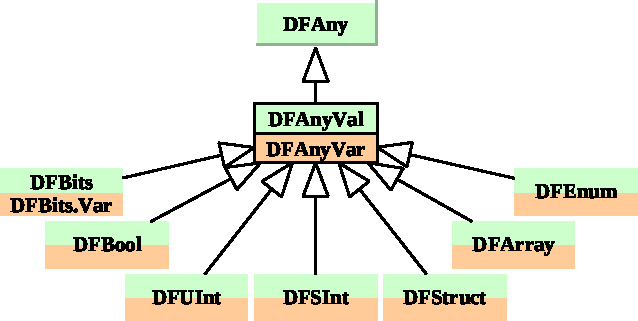
\includegraphics[scale=0.7]{graphics/Inherit.pdf} 
%	\captionof{figure}{DFiant dataflow types: simplified inheritance diagram}
%	\label{fig:Inherit}
%\end{figure}

\subsection{Dataflow Semantics}
DFiant has a dataflow programming model. Data scheduling order, or \textit{token-flow}, is set by the \textit{data dependency}. Essentially, the DFiant semantics schedules all independent dataflow expressions concurrently, while dependent operations are synthesized into a guarded FIFO-styled pipeline. Dataflow branches are implicitly forked and joined. Unused nodes, semantically, always consume tokens, and are discarded during compilation. We observe the DFiant \code{f} implementation as follows:

\begin{enumerate}
  \item All expressions are dataflow variable declarations.
  \item Concurrency is implicit, and \code{f} is coded intuitively, in a sequential manner, since dataflow dependency is oblivious to statement order. 
  \item All scheduling is implicitly guarded by its dependencies. For example, \code{a} is forked into both \code{b} and \code{c} operations, while \code{c} joins branches from \code{a} and \code{b}.
  It is impossible to read an invalid result or an old result (without extending semantics further).
  \item DFiant semantics are intuitive: data is consumed only when it is ready and can be accepted by all receiving nodes, while back-pressure prevents data loss. 
\end{enumerate} 

%The basic DFiant types are DFBits and DFBool
%Each dataflow type points to a static bits vector
%As can be seen from Related Work, HLS "LO TAFAS". Fig. \ref{boxy}
%WE believe one of the primary reasons is that missing features of RTL
%In this section we will cover the RTL features of RTL and how they handled in DFiant's abstractions
%Bring type driven development into hardware design.
%Need inheritance tree.
%Interactions with scala types


\subsection{Bit-Accurate Operations, Type Inference, and Data Structures}
All DFiant's dataflow types are bit-accurate and structurally static, with their bit-width set upon construction (e.g., \code{DFBits[5]} is a 5-bit vector). Operations between dataflow variables produce a bit-accurate result with the proper type inference. For example, an addition between an unsigned 5-bit variable (\code{DFUInt[5]}) and a signed 10-bit variable (\code{DFSInt[10]}) produces an adder that can be implicitly converted to a 10-bit signed variable, if carry is not required, or an 11-bit signed variable by explicitly invoking \code{.wc} from the addition.

DFiant also allows operations between dataflow types and their corresponding Scala numeric types, by treating the Scala numeric types as constants (e.g., addition between \code{DFSInt} and \code{Integer} variables). A constant in the dataflow graph is a node that can produce infinite tokens of the same value.   

\subsection{Mutability}
\label{sec:mutability}
DFiant supports dataflow variables mutability via the \code{:=} operator. Do not confuse with Scala-level mutability which is enabled by using \code{var} instead of \code{val}. Each dataflow class has two variations: an immutable class, which inherits from \code{DFAny\textbf{Val}} and a mutable class, which inherits from \code{DFAny\textbf{Var}} and accepts \code{:=}. The difference between the types enforces an immutable right-hand-side (RHS), where required, and a mutable variable creation. Consider, for instance, the DFiant implementation of \code{g} in Table \ref{tbl:StateExDefImpl}: \code{a} is immutable because it is a RHS addition between the dataflow variable \code{i} and a literal value \code{5}. Contrarily, \code{c} is mutable, since it is a dataflow variable constructor (\code{.init} constructs a new initialized variable, while preserving the mutability trait). 

Fig.~\ref{fig:Inherit} demonstrates a dual class definition for every type  (immutable and mutable). The naming convention helps to reason about the mutability. For example, \code{DFBits} and \code{DFBits.Var} are immutable and mutable classes, respectively. Constructing a new variable via \code{DFBits} (e.g, \code{val a = DFBits[5]}) returns the mutable \code{DFBits.Var[5]}. Usually, we either receive or return an immutable type, hence we do not require annotating a type with its mutable variation. In cases where we want to return a mutable type, we annotate it as an output port (see Section~\ref{sec:io_ports}).

%DFiant's code safety is enforced by maintaining the 'DF-mutability' trait while aliasing (accepting the ':=' operator). This means that an alias of a \textbf{Var}, is still a \textbf{Var}, and can be assigned, while an alias of a \textbf{Val} cannot. This concept is illustrated in ???, and further explained in ???:




\subsection{Bit Aliasing and Casting}
Aliasing in DFiant enables referencing a part of a dataflow variable, by invoking \code{.bits(hiIdx, loIdx)}, which creates a bits vector alias that references the original variable at the given index parameters. Every change of a dataflow variable affects its alias and vice versa (similar to VHDL's signal aliasing). Since this function also casts the variable as \code{DFBits}, this feature is used as a raw-data cast between different dataflow types. Aliasing of an alias is also possible, while maintaining relative bits indexing. Aliasing preserves the mutability trait: an alias of an immutable variable is immutable, while an alias of a mutable variable is mutable. 


Fig.~\ref{fig:Aliasing} demonstrates aliasing code and its effect on the contents of a dataflow variable (\code{bits128}). Each line code does as follows:
\begin{enumerate}
  \item Constructs a new 128-bit vector, \code{bits128}, and clears it.
  \item Creates a new alias, \code{alias64}, which references the most significant 64 bits of \code{bits128}. Since \code{bits128} is a \code{DFBits} variable, there is no need to invoke \code{.bits()}, and we can apply the required indexes directly.
  \item Creates a new alias, \code{alias32}, which references the least significant 32 bits of \code{alias64}, which reference bits 64 to 95 of \code{bits128}.
  \item Constructs a new double precision floating point dataflow variable, \code{dbl}, and initialize its value as \code{1.0} (hexadecimal value of \code{0x3FF00...0}).
  \item Modifies the least significant byte of \code{dbl}.
  \item Sets the most significant bit of \code{bits128}.
  \item Assigns \code{dbl} to the least significant 64 bits of \code{bits128} through casting. All the bits of \code{dbl} are selected because \code{.bits()} is invoked without index parameters.
  \item Modifies a byte of \code{bits128}.
  
\end{enumerate}

\begin{figure}[h]
  \centering
  \begin{minipage}[b][3cm][b]{0.57\linewidth}
    \vfill
    \begin{minted}[xleftmargin=1.5em,linenos,autogobble,tabsize=2,framesep=1pt, frame=single,fontsize=\fontsize{8}{8}\selectfont]{scala}
      val bits128 = DFBits[128] := 0
      val alias64 = bits128(127, 64)
      val alias32 = alias64(31, 0)
      val dbl = DFDouble := 1.0
      dbl.bits(7,0) := 0x28
      bits128(127) := 1
      bits128(63, 0) := dbl.bits()
      alias32(16, 8) := 0x57		    
    \end{minted}
    \vfill
    \subcaption{DFiant code}
  \end{minipage}%
  \hfill
  \begin{minipage}[b][3cm][b]{0.42\linewidth}
    \centering
    \vfill
		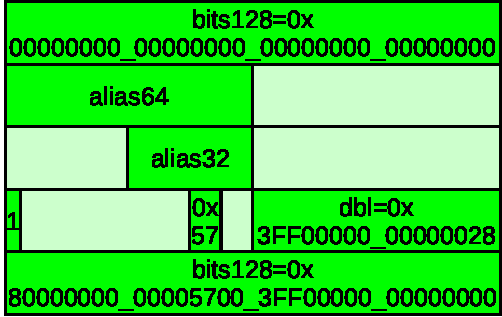
\includegraphics[width=\linewidth]{graphics/Aliasing.pdf} 
    \vfill
    \subcaption{Contents of \code{bits128}}
  \end{minipage}
  \captionof{figure}{Bit aliasing and casting example}
  \label{fig:Aliasing}
\end{figure}


\subsection{Structural Composition and Generation}

DFiant expands traditional structural composition capabilities by utilizing Scala's object oriented features such as inheritance and polymorphism, as well as finite loops and recursive composition. The hierarchical compositions provide the scope and dependencies for the dataflow variables. The hierarchy itself is transparent to the dataflow graph, as if the entire design is flattened, inlined, and unrolled. Therefore, hierarchies in DFiant are synthesizable, highly reusable, and do not affect the design performance (may affect compilation time). Different composition examples are available in Table~\ref{tbl:Box}.

\begin{table*}[t]
  \captionof{table}{DFiant Hierarchy Example: Inheritance, Polymorphism, Recursive Composition, and Inlined View}
  \label{tbl:Box}
  \begin{tabular}{|c|c|c|}
    \hline 
    \textbf{Description} & \textbf{DFiant Code} & \textbf{Functional Drawing} \\ 
    \hline
    \begin{minipage}{0.1\textwidth}
      \footnotesize
      \flushleft
      Abstract base class, \code{Box} (defines only an interface)
    \end{minipage} 
    &
    \begin{minipage}{0.48\textwidth}
      \begin{minted}[autogobble,tabsize=2,framesep=1pt,fontsize=\fontsize{8}{8}\selectfont]{scala}
      type DFB = DFUInt[32] //Type alias, to save code space
      abstract class Box(iT: DFB, iB: DFB) { //T=Top, B=Bottom 
        val oT: DFB
        val oB: DFB
      }
      \end{minted}
    \end{minipage} 
    &  
    \begin{minipage}[c][1.5cm]{0.34\textwidth}
      \centering
      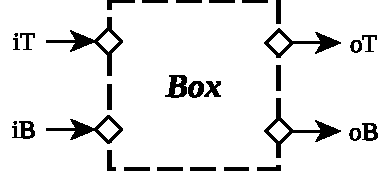
\includegraphics[height=1.3cm]{graphics/Box.pdf}%
    \end{minipage} 
    \\ 
    \hline 
    \begin{minipage}{0.1\textwidth}
      \footnotesize
      \flushleft
      Concrete \code{Box} implementation examples
    \end{minipage} 
    &
    \begin{minipage}{0.48\textwidth}
      \begin{minted}[autogobble,tabsize=2,framesep=1pt,fontsize=\fontsize{8}{8}\selectfont]{scala}
      case class BoxY(iT: DFB, iB: DFB) extends Box(iT, iB) {
        val (oT, oB) = (iT * iT, iT + iB)
      }
      case class BoxE(iT: DFB, iB: DFB) extends Box(iT, iB) {
        val (oT, oB) = (iT + iB, iB)
      }
      \end{minted}
    \end{minipage} 
    &  
    \begin{minipage}[c][1.8cm]{0.34\textwidth}
      \centering
      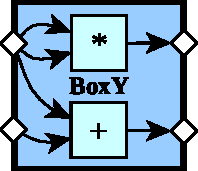
\includegraphics[height=1.3cm]{graphics/BoxY.pdf}%
      \quad\quad\quad
      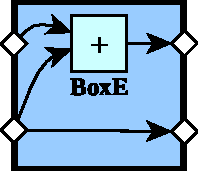
\includegraphics[height=1.3cm]{graphics/BoxE.pdf}%
    \end{minipage} 
    \\ 
    \hline
    \begin{minipage}{0.1\textwidth}
      \footnotesize
      \flushleft
      \code{Box123}, an abstract polymorphic composition of three \code{Box} instances
    \end{minipage} 
    &
    \begin{minipage}{0.48\textwidth}
      \begin{minted}[autogobble,tabsize=2,framesep=1pt,fontsize=\fontsize{8}{8}\selectfont]{scala}
      abstract class Box123(iT: DFB, iB: DFB) extends Box(iT, iB){
        def b1Bld(iT: DFB, iB: DFB) : Box
        def b3Bld(iT: DFB, iB: DFB) : Box
        val b1 = b1Bld(iT,     iB)
        val b2 = BoxE(b1.oB,   b1.oT)
        val b3 = b3Bld(b2.oB,  b2.oT)
        val (oT, oB) = (b3.oT, b3.oB)
      }
      \end{minted}
    \end{minipage} 
    &  
    \begin{minipage}[c][2.3cm]{0.34\textwidth}
      \centering
      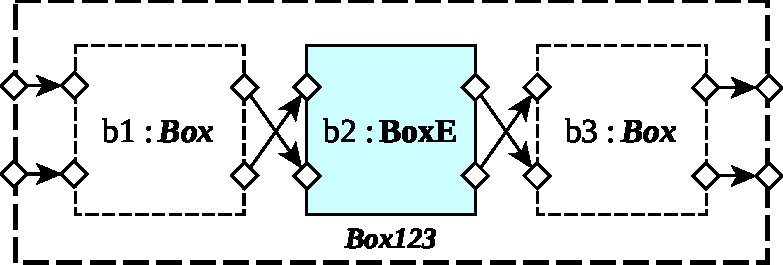
\includegraphics[height=2.1cm]{graphics/Box123.pdf}%
    \end{minipage} 
    \\ 
    \hline
    \begin{minipage}{0.1\textwidth}
      \footnotesize
      \flushleft
      \code{BoxYEE}, a concrete polymorphic composition of three \code{Box} instances \\+\\An inlined view of \code{BoxYEE}
    \end{minipage} 
    &
    \begin{minipage}{0.48\textwidth}
      \begin{minted}[autogobble,tabsize=2,framesep=1pt,fontsize=\fontsize{8}{8}\selectfont]{scala}
      case class BoxYEE(iT: DFB, iB: DFB) extends Box123(iT, iB) {
        def b1Bld(iT: DFB, iB: DFB) = BoxY(iT, iB)
        def b3Bld(iT: DFB, iB: DFB) = BoxE(iT, iB)
      }
      \end{minted}
    \end{minipage} 
    &  
    \begin{minipage}[c][4.6cm]{0.34\textwidth}
      \centering
      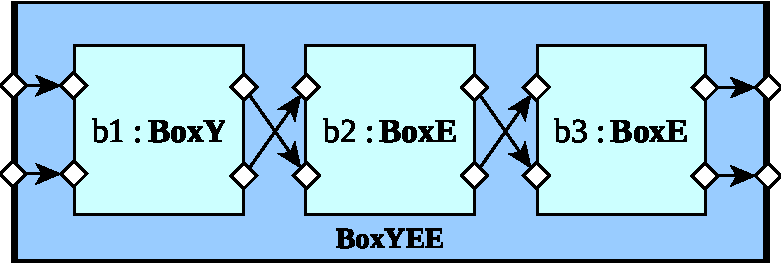
\includegraphics[height=2.1cm]{graphics/BoxYEE.pdf} \\
      \vspace{0.1cm}
      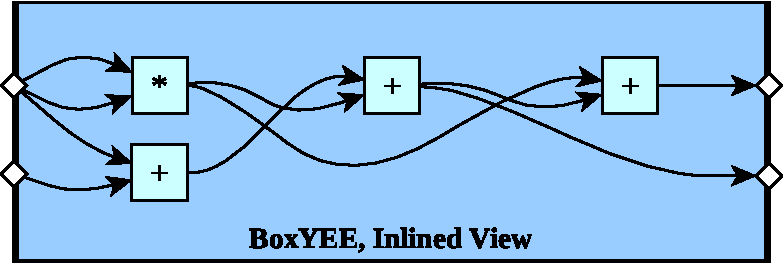
\includegraphics[height=2.1cm]{graphics/BoxYEEInlined.pdf}%
    \end{minipage} 
    \\ 
    \hline
    \begin{minipage}{0.1\textwidth}
      \footnotesize
      \flushleft
      Finite recursive composition example
    \end{minipage} 
    &
    \begin{minipage}{0.48\textwidth}
      \begin{minted}[autogobble,tabsize=2,framesep=1pt,fontsize=\fontsize{8}{8}\selectfont]{scala}
      case class BoxBox(N: Int)(iT: DFB, iB: DFB) 
      extends Box(iT, iB) {
        val b = BoxY(iT, iB)
        val bb : Box = if (N > 0) BoxBox(N - 1)(b.oT, b.oB)
                       else b
        val (oT, oB) = (bb.oT, bb.oB)
      }
      \end{minted}
    \end{minipage} 
    &  
    \begin{minipage}[c][2.3cm]{0.34\textwidth}
      \centering
      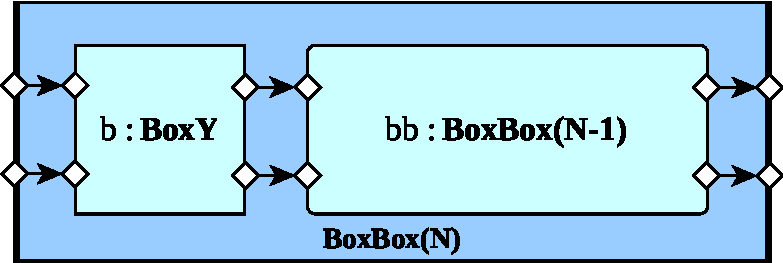
\includegraphics[height=2.1cm]{graphics/BoxBox.pdf}%
    \end{minipage} 
    \\ 
    \hline
  \end{tabular} 
\end{table*}


\subsection{IO Ports}
\label{sec:io_ports}
The class \textit{Box} from Table~\ref{tbl:Box} can also be coded as demonstrated in Fig.~\ref{fig:IOBox}. The annotation \code{DFVar $<>$ Dir} controls \textit{DFVar}'s access by encapsulating the variable with the dataflow port class, \code{DFPort}: an \code{IN} port can only be read (immutable), while an \code{OUT} port can only be modified (unreadable). DFiant has implicit conversions in place that selectively converts between \code{DFPort} and \code{DFAny} instances, without breaking mutability rules and type safety. The port annotations match the capabilities of traditional HDLs, and are noticeably absent from HLS languages such as C++. 


\begin{figure}[h]
  \centering
  \begin{minipage}{0.4\linewidth}
  \begin{minted}[autogobble,tabsize=2,framesep=1pt, frame=single,fontsize=\fontsize{8}{8}\selectfont]{scala}
  abstract class Box() { 
    val iT: DFB <> IN
    val iB: DFB <> IN
    val oT: DFB <> OUT
    val oB: DFB <> OUT
  }
  \end{minted}
  \end{minipage}
  \captionof{figure}{IO port annotation DFiant code example}
  \label{fig:IOBox}
\end{figure}



%+ C has no clear input/output notation. Input array and output array are the same.
%
%+ IDE: Intellisense, error highlighting, code completion, watches, println.
%+ Unified compilation
%+ Complete project build with the IDE. Compile results.
%Yes abstract away pipelining. No to scheduling control.
%
%Features we don't want
%simulations constructs.
%separate constraints file.
%
%VHDL Possible race conditions.
%
%
%+Include a summary table of RTL feature abstraction and how their are defined in DFiant.


\section{The DFiant Compiler}

\section{Proof of Concept}
\label{sec:evaluation}
In this section we demonstrate DFiant frontend and backend compilers as a proof of concept the preliminary semantics of DFiant by implementing two case studies: an AES cypher, and a double precision FPMul. We compare both test cases against traditional designs, and demonstrate competing performance while simplifying code verbosity significantly. 

\subsection{Methodology}
We implemented both test cases in DFiant, constrained them by a variance of minimum frequency requirements, and compiled them to RTL. The DFiant compiler automatically pipelined the design to achieve the required minimum frequency, and generated an RTL verilog file and a TCL constraints file. For a baseline we obtained equivalent open-source RTL cores and Vivado HLS implementations, where possible. We disabled the DFiant backend support for pipelined valid/ready signaling and a blocking back-pressure, since the RTL cores did not support this capability.

We chose the following comparison metrics: the maximum clock frequency, clock cycle latency, utilizations of both look-up tables (LUTs) and flip-flop registers (FFs), and lines of code (LoC). Digital signal processing (DSP) block utilization was zero for AES and equivalent for FPMul across all designs, thus neglected from the table. a We used Xilinx Vivado to synthesize and implement the RTL design for a Virtex-7 FPGA, part number: xc7vx485tffg1761-2. The tool was configured to use default strategy for both synthesis and implementation processes. For each design, we recorded the maximum clock frequency, LUTs, and FFs. We recorded the design latency as reported by the DFiant and Vivado HLS compilers, and the RTL cores documentation. Finally, we automatically counted the LoC \cite{danial2009cloc}, applied standard score normalization (0-100) to all metrics, and assured higher values indicate better score for all metrics. Mean score of all metrics is presented as well.

\subsection{Case Study: AES Cypher}
For baseline comparison we used three AES cypher RTL designs from opencores.org: Das core \cite{das2010fully}, Hsing core \cite{hsing2013aes} and Salah core \cite{salah2013aespipe}. Additionally, we obtained a Vivado C++ HLS design~\cite{oflynn2014rapid}. All these designs are fully pipelined, meaning that in every cycle the design accepts new key and data inputs, and emits an encrypted data output, delayed by a fixed design latency.

We compiled the DFiant and Vivado HLS designs with three target clock frequencies: 200 MHz, 300 MHz, and 450 MHz. We named the designs accordingly (e.g., DFiant\_200 is the 200MHz target design). We collected the results in Table~\ref{tbl:AES_Compare_Table}, and displayed their normalized standard score in Fig.~\ref{fig:AES_Compare_Graph}. We added the supported key types quantity as a metric, since some designs support 128bit keys and do not include 192bit and 256bit keys as well. The table also includes an 'SBox BRAM Use' column, since some designs do not use memory to implement the AES SBox function.

\begin{table*}[t!]
  \centering
  \begin{minipage}[t][5cm][t]{0.62\linewidth}
    \centering
    \captionof{table}{AES Cypher RTL Designs Comparison\\(the numbering on the left associates configurations with \fig{fig:AES_Compare_Graph})}
    \label{tbl:AES_Compare_Table}
    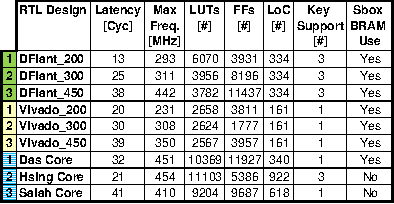
\includegraphics[scale=1]{graphics/AES_Compare_Table.pdf} 
  \end{minipage}
  \hfill
  \begin{minipage}[t][5cm][t]{0.37\linewidth}
    \centering
    \captionof{table}{FP Mult. RTL Designs Comparison\\(the numbering on the left associates configurations with \fig{fig:FP_Compare_Graph})}
    \label{tbl:FP_Compare_Table}
    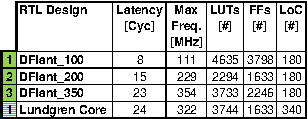
\includegraphics[scale=1]{graphics/FP_Compare_Table.pdf} 
  \end{minipage}
  \begin{minipage}[b][3.8cm][b]{0.62\linewidth}
  	\centering
    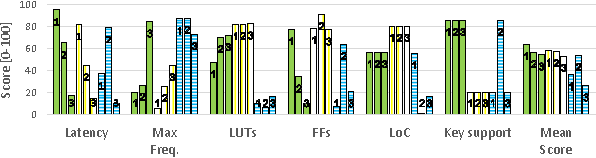
\includegraphics[height=3cm]{graphics/AES_Compare.pdf} 
    \captionof{figure}{AES cypher RTL designs score comparison (higher = better)\\ \quad}
    \label{fig:AES_Compare_Graph}
  \end{minipage}
  \hfill
  \begin{minipage}[b][3.8cm][b]{0.37\linewidth}
    \centering
    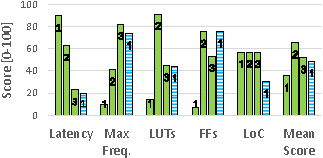
\includegraphics[height=3cm]{graphics/FP_Compare.pdf} 
    \captionof{figure}{FP multiplication RTL designs score comparison (higher = better)}
    \label{fig:FP_Compare_Graph}
  \end{minipage}
\end{table*}

The Hsing core clearly has the best performance among the different designs (but the lowest score on LUTs utilization). The primary reason it achieved this is because it uses LUTs instead of BRAMs. This enables the synthesizer to optimize the AES SBox function, and even pipeline it. DFiant uses its \code{lookupTable} library function to implement SBox, and we have yet to enable such an option for DFiant. 

Although the DFiant-generated RTL performance is not optimal, it can still  be improved without modifying the DFiant AES code, if the DFiant compiler is optimized. Moreover, this code has an adaptive pipeline, while the RTL cores pipelines are fixed. The Vivado implementation enjoys the same advantages as DFiant, and has even less LoC. However, the Vivado code does not support all possible keys and its maximum performance is far from optimum (we did not attempt to improve the HLS pragma directives).

If we assume all metrics have the same weight, the mean score places the DFiant solutions at the top. It is difficult to determine what is truly the best solution, but DFiant clearly has the best potential for further improvement without any modification to the application code.

           
\subsection{Case Study: Double Precision FPMul}

We compared our FPMul with the open IEEE-754 compatible Lundgren core \cite{lundgren2014open} (the only IEEE-754 fully compatible FPMul RTL design we had access to). Since the core is a complete floating point unit, we disabled the unnecessary parts, reducing it to only an FPMul, for a fair comparison with DFiant's code. The DFiant code was written by using the Lundgren VHDL code as a reference design. The designs are very similar in their structure, except that DFiant is considerably less verbose, and has no explicit pipeline.

We had no access to an open Vivado HLS FPMul for comparison. We could have directly invoked a \textit{double} multiplication, but an inspection of the generated RTL revealed that Vivado HLS just instantiates an RTL floating point blackbox core. DFiant can choose to use this core as well, and achieve identical performance to Vivado HLS. Furthermore, the Vivado HLS floating point implementation is not fully compatible with IEEE-754 (e.g, does not support denormalized numbers).

Similarly to the AES case study, we collected the results in Table~\ref{tbl:FP_Compare_Table}, and displayed their normalized standard score in Fig.~\ref{fig:FP_Compare_Graph}. In comparison with the Lundgren core, DFiant\_350 is better in every criteria, aside from FFs utilization. Ultimately, DFiant out-performs its reference design of FPMul, and demonstrates its ability to provide different RTL designs for design space exploration.


\section{Conclusion}
\label{sec:conclusion}
In this paper we presented our extension of DFiant, a dataflow HDL, and exposed its advantageous semantics, when compared to modern RTLs and C++-based HLS tools, such as VHDL and Vivado HLS, respectively. DFiant provides a seamless concurrent programming approach, and yet it still facilitates a versatile compositional and hierarchical expressiveness. We evaluated DFiant in two computational-heavy case studies, and demonstrated its competing performance alongside its code simplification. 

%Although we established its many benefits, DFiant is still missing a few milestones before it becomes a worthy replacement for the traditional HDLs. 
So far,  we demonstrated how DFiant covers static one-to-one token transfer functions. Notwithstanding, functionality may require upsampling (e.g., duplicate each token), downsampling (e.g., drop every third token), token arrival time dependency (e.g., priority round-robin arbiter), or token value dependency (e.g., filter out odd-valued tokens). Future work may explore expanding control over token generation and consumption.

%%%%%%%%%%%%%%%%%%%%%%%%%%%%%%%%%%%%%%%%%%%%%%%%%%%%%%%%%%%%%%%%%%%%%%%%%%%%%%%%%%


%%%%%%%%%%%%%%%%%%%%%%%%%%%%%%%%%%%%%%%%%%%%%%%%%%%%%%%%%%%%%%%%%%%%%%%%%%%%%%%%%%
% Acknowledgement
%%%%%%%%%%%%%%%%%%%%%%%%%%%%%%%%%%%%%%%%%%%%%%%%%%%%%%%%%%%%%%%%%%%%%%%%%%%%%%%%%%
%%
%% The acknowledgments section is defined using the "acks" environment
%% (and NOT an unnumbered section). This ensures the proper
%% identification of the section in the article metadata, and the
%% consistent spelling of the heading.
%\begin{acks}
%LEGaTO ack here
%\end{acks}
%%%%%%%%%%%%%%%%%%%%%%%%%%%%%%%%%%%%%%%%%%%%%%%%%%%%%%%%%%%%%%%%%%%%%%%%%%%%%%%%%%


%%%%%%%%%%%%%%%%%%%%%%%%%%%%%%%%%%%%%%%%%%%%%%%%%%%%%%%%%%%%%%%%%%%%%%%%%%%%%%%%%%
% Bibliography
%%%%%%%%%%%%%%%%%%%%%%%%%%%%%%%%%%%%%%%%%%%%%%%%%%%%%%%%%%%%%%%%%%%%%%%%%%%%%%%%%%
%%
%% The next two lines define the bibliography style to be used, and
%% the bibliography file.
\bibliographystyle{ACM-Reference-Format}
\bibliography{bib/macros,bib/references}
%%%%%%%%%%%%%%%%%%%%%%%%%%%%%%%%%%%%%%%%%%%%%%%%%%%%%%%%%%%%%%%%%%%%%%%%%%%%%%%%%%



\end{document}
\endinput